\chapter{Introduction}
\label{chap:intro}

% Intro: slightly more than 30 pages in a review form, and set up framework (topics and challenges) for the projects

% Cancer
% mutation
% Multi-omics

% PTM
% heterogeneity
% tumor microenvironment
% precision medicine


% Large scale patient samples collection (consoritum works)

% data portal

% data sharing
% pipeline execution
% gene annotation
% integration


% GBM

% Outline of the dissertation


\section{Cancer and precision medicine}
Cancer is the leading cause of death in most countries in the world \cite{sungh_brayf:GlobalCancer2021}. In the U.S., cancer is estimated to introduce roughly 1.9 millions cases and 600 thousands deaths in 2021, where \textasciitilde40\% of the population will be diagnosed with cancer at some point in their lifetime \cite{siegelrl_jemala:CancerStatistics2021}. Despite advancements in understanding and treating cancer in the past 50 years, many forms of the disease lack effective treatment, and how normal cells become cancerous and form a tumor, the process known as oncogenesis, remains to be fully deciphered. Therefore, the cancer research community continues to work on better characterization of cancer and its treatment as our ultimate goals.

The functional properties of a tumor have been described as ``cancer hallmarks'' \cite{hanahand_weinbergra:HallmarksCancer2011}, including cell proliferation, immortality in replication, cell death evasion, and increased ability of angiogenesis and invasion. While the tumor microenvironment, the surrounding tissue environment where a tumor develops, consists of normal cells, the tumor microenvironment also helps maintain tumor abbrent growth and immune respones beneficial to the tumors \cite{hanahand_weinbergra:HallmarksCancer2011,quaildf_joyceja:MicroenvironmentalRegulation2013}. To develop an effective cancer treatment, it's important to understand how cancer hallmarks are achieved during the oncogenesis and the complicated cell-cell interactions in the tumor microenvironment.


\subsection{Oncogenesis and the functional impact of somatic mutation}
Oncogenesis is currently viewed as a microevolution process where normal cells acquire somatic mutations that offer growth and survival advantage \cite{strattonmr_futrealpa:CancerGenome2009,martincorenai_campbellpj:SomaticMutation2015}. The somatic mutation rate in human is estimated to be about 2 to 10 mutations per cell division \cite{lynchm_lynchm:RateMolecular2010,milhollandb_vijgj:DifferencesGermline2017}. A tumor may accumulate 0.01--100 mutations per megabase in the genome depending on the cancer type \cite{lawrencems_getzg:MutationalHeterogeneity2013,martincorenai_campbellpj:SomaticMutation2015}. However, only some of the mutations might confer a growth and survival advantage while remaining mutations are either benign or of unknown phenotype. Such actively selected mutations are frequently found in certain genes, known as cancer driver genes and significantly mutated genes (SMGs) \cite{dingl_mariamidzea:PerspectiveOncogenic2018}. There are three main types of cancer driver genes: proto-oncogenes that promotes cell growth, tumor suppressor genes that regulate cell growth, and DNA rapair genes that fix DNA damages.

Mutations in one cancer gene or a combination of them are sufficient to drive the oncogenic process. For example, transcription factor \gene{TP53} is a tumor suppressor gene\footnotemark{} and it responds to DNA damage by inducing cell cycle arrest \cite{kastanmb_craigrw:ParticipationP531991}. Mutations in TP53 can lead to the uncontrolled proliferation of mutated cells, thereby causing cancer. Thus, \gene{TP53} is one of the most commonly found cancer genes in a tumor, whose mutations can be found in a remarkable 37.5\% of over 9 thousands tumor samples examined across 33 cancer types \cite{baileymh_dingl:ComprehensiveCharacterization2018}. On the other hand, \gene{EGFR}, epidermal growth factor receptor, is a well known proto-oncogene that encodes a transmembrane protein that activates cell signaling pathways to promote cell growth. The mutations in \gene{EGFR} often lead to increased gene expression or uncontrolled activation of its function, and are commonly found in breast, lung, and brain cancer patients \cite{ciardiellof_tortorag:EGFRAntagonists2008}.

\footnotetext{\gene{TP53}'s role as a cancer drive gene is complicated. While the majority of its mutations are loss-of-function, leading to decreased ability to suppress tumor growth, it also exhibits oncogene properties with gain-of-function mutations \cite{petitjeana_olivierm:TP53Mutations2007}.}

Therefore, characterizing the functional impact of a mutation has been an area of intensive research ever since the first cancer somatic mutation was identified in \citeyear{reddyep_barbacidm:PointMutation1982} \autocite{reddyep_barbacidm:PointMutation1982,tabincj_changeh:MechanismActivation1982}. Besides well controlled experimental validation, a number of statistical methods have been widely-used to infer functional elements, including high gene mutation rate, mutation recurrence, mutual exclusivity, and co-occurrence of mutations across multiple samples or cancer types, since these phenomena imply positive selection \cite{martincorenai_campbellpj:SomaticMutation2015}. However, only a few mutations are well understood and the majority of them have unknown function in cancer. Even for well-known cancer driver genes like \gene{PIK3CA} and \gene{BRCA1/2}, only a fraction of suspected cancer-related mutations having actually been functionally validated \cite{ngpks_millsgb:SystematicFunctional2018}. It is still challenging today to attribute a phenotypic ``cancer hallmark'' expressed by a tumor to its mutations.


\subsection{Multi-omics portrait of cancer}
Since the phenotypes of cancer hallmarks are achieved through abberant alterations at multiple molecular levels, a new paradigm to understand complex diseases like cancer is through the lens of multi-omics analysis \cite{deanda-jaureguig_hernandez-lemuse:ComputationalOncology2020}. Thanks to the recent advancements in high-throughput experiments (commonly termed ``omics''), we are able to profile the specimen systematically at a molecular level. Common omics assays include:

\tightlists
\begin{itemize}
    \tightlist
    \item Genomic: whole exome sequencing, whole genome sequencing
    \item Transcriptome: RNA sequencing, miRNA sequencing
    \item Epigenomics: DNA methylation microarray, whole genome bisulfite sequencing, ChIP-seq, ATAC-seq
    \item Proteomics: TMT multiplexed mass spectrometry
    \item Single cell omics: single cell/nuclei RNA and ATAC sequencing
    \item Imaging: Imaging mass cytometry, CODEX, histopathology H\&E slides
    \item Spatial transcriptomics: 10x Genomics Visium
\end{itemize}

By investigating the biological signals and features accquired from different molecular assays in the same specimen, we are able to ``connect the dots'' and reason how a genetic alteration contributed to the phenotypes, furthermore, how a set of genetic alterations interact together. For example, \gene{EGFR} is an oncogene commonly altered in glioblastoma \cite{eskilssone_miletich:EGFRHeterogeneity2018}, but we are unsure of its functional impace. Using multi-omics approach, we will be more confident to attribute the cell profileration of a glioblastoma to genetic alterations in \gene{EGFR} if we are able to pick up concordant findings from different experiment assays: mutation or amplification of \gene{EGFR} is detected; RNA expression, protein abundance, and activating phosphorylation of EGFR are all increased in this sample relative to the wild-type tumors and normal samples; increased activity in the RTK-RAS-MAPK pathway; single cell and imaging omics showing the increased EGFR activity is found in tumor cells and not normal cells in the tumor microenvironment. Multi-omics analysis allows us to model the complex biological phenomenon as systems consisted of complicated interactions, which allows us to protray the relatively abstract activities of cancer hallmarks by mapping all the abberant activities integratively.

Conducting multi-omics characterization of cancer naturally calls for large scale collaborations since it requires more samples to power statistical modeling and requires different expertise to carry out diverse experimental assays and data integration. As a result, more consortia and large-scale projects are founded as the foundation for multi-omics studies \cite{hutterc_zenklusenjc:CancerGenome2018,rozenblatt-roseno_zhuangx:HumanTumor2020,rodriguezh_lowydr:NextHorizon2021}.


\subsection{Precision medicine}

% Due to the random nature of oncogenesis, each tumor is different in their mutational profile.


% Our lab has also studied the effect of coding mutations on protein structure \autocite{niu_protein-structure-guided_2016}. \citeauthor{niu_protein-structure-guided_2016} found that mutations cluster spatially in the functional protein domains of driver genes. For example, mutations clustering near an EGFR phosphotyrosine site in the 3D tertiary structure have been shown to increase autophosphorylation levels and EGFR activity \autocite{niu_protein-structure-guided_2016}.

% Many somatic mutations have unknown significance; transition to PTM
%  Since post-translational modifications (PTMs) are known to be essential for signal transduction \autocite{hunter_signaling2000_2000}, I propose to explore the functional impacts of mutations by investigating their effects on PTMs.


% TODO: need a section to describe TCGA, CPTAC and HTAN

\section{Computational challenges in large-scale multi-omics studies}
Large scale multi-omics studies produce massive amount of data, providing insights into complicated biological systems and allowing researchers to generate hypotheses from their research angle. However, they also introduce a new set of computational challenging that impeding the usability of the data by the research community. First,

% FAIR guideline foundational principles: Findability, Accessibility, Interoperability, and Reusability

GDC\cite{heathap_grossmanrl:NCIGenomic2021}
% Pipeline standardization
% Data management
% gene annotation difference
%     gene symbol
%     gene version
%     annotation across different data types
% integration

FAIR guideline \cite{wilkinsonmd_monsb:FAIRGuiding2016}


Here we focus on the computational challenges for studies that have a standardized set of experiment techniques and protocols. However, there are additional obstacles in integrating data of the same molecular type but by different protocols. For example, RNA-seq using polyA enriched and ribosomal RNA depletion protocols captures different RNA species and may different variations in the expression quantification \cite{cuip_yuj:ComparisonRibominus2010,chenl_chenl:PairedRRNAdepleted2020}. Phosphoproteomics generated by different mass spectrometry strategies (e.g., MS2 and MS3 spectra) have greatly variable ability to identify phosphopeptides and different dynamic ranges in the quantification \cite{ulintzpj_nesvizhskiiai:ComparisonMS2only2009}. The existing data repositories like GDC and SRA do not automatically remove the batch effect introduced by the different experiment protocols, so it is up to the users to apply extra care and computational approaches to determine the severity of such batch effect and the approach of batch effect removal.

Gene naming \cite{fujiyoshik_oginos:OpinionStandardizing2021}
\cite{brufordea_tweedies:GuidelinesHuman2020}


\section{Post-Translational modifications (PTM) in cancer}
% Post-translational modifications (PTMs) dynamically regulate protein function through the covalent addition of chemical moieties to nascent polypeptides following translation. Common PTM types in humans include phosphorylation, acetylation, and ubiquitination, having distinct roles in regulating protein function. Notably, phosphorylation of adaptor proteins by kinases can potentiate intracellular signaling, while histone acetylation by acetyltransferases can affect chromatin architecture. Alternatively, lysine polyubiquitination by ubiquitin ligases can promote proteasomal degradation of substrate proteins.

% Phosphorylation is the most common PTM in human cells, occurring primarily on serine (61.8\%), threonine (24.0\%), and tyrosine (14.2\%) residues \autocite{hornbeck_phosphositeplus:_2012}. Kinases and phosphatases catalyze the reversible addition and removal of phosphate groups, respectively, which can amplify or dampen signal transduction. Phosphorylation tightly regulates cell signaling pathways through the dynamics of kinases and phosphatases.

% Acetylation, ubiquitination and methylation also play important roles in signaling transduction and gene regulation. Acetylation refers to the process where the acetyl group from acetyl-coenzyme A (acetyl-CoA) is transferred to the $\varepsilon$-amine of a lysine residue \autocite{ali_lysine_2018}. Importantly, histone acetylation can remodel chromatin at the promoter region of actively transcribed genes \autocite{suganuma_signals_2011}, which dynamically modifies chromatin architecture and “opening” genomic DNA. Lysine acetylation on non-histone proteins has also been investigated. For example, CBP (\gene{KAT3A}) and p300 (\gene{KAT3B}) acetylate and activate p53 through promoting its DNA-binding affinity \autocite{scolnick_creb-binding_1997,brooks_impact_2011}. Conversely, p53 can be deacetylated and inactivated by lysine deacetylases (KDACs), such as sirtuin 1 (\gene{SIRT1}) and HDAC1 \autocite{brooks_impact_2011,luo_deacetylation_2000}.

% Ubiquitination involves the addition of the small protein ubiquitin to a lysine residue of the protein substrate, which can mark the substrate for degradation by the proteasome \autocite{komander_ubiquitin_2012}. Ubiquitination is also capable of altering the cellular location and function of a substrate \autocite{mukhopadhyay_proteasome-independent_2007}\autocite{schnell_non-traditional_2003].



\section{Glioblastoma}
GBM is the most common primary malignant brain tumor with an incidence of 3.22 per 100,000 persons in the United States, a median survival of less than 2 years from diagnosis18,19 and limited treatment options20,21. TCGA surveyed 206 GBMs with genomic and transcriptomic profiling22, extending the subclassifications developed by Aldape and colleagues23,24. The current view is that IDH-wild type GBMs fall into three distinct subclasses: proneural, classical, and mesenchymal, based on genomic alterations and gene expression signatures22,24–28. The tumor microenvironment may also play an important role in GBM pathogenesis, where tumor-associated macrophages (TAMs) comprise the majority of the immune population29–31. TAMs originate from tissue-resident microglia and bone marrow-derived macrophages (BMDMs), with evidence suggesting that they facilitate tumor proliferation, survival, and migration30. M2-type macrophages, typically thought of as immunosuppressive, dominate and may serve as a microenvironmental advantage to the tumor32.

Despite extensive molecular and immunological characterization of GBM, surgical resection followed by concurrent chemotherapy and radiotherapy remain the standard of care33–35, and targeted therapies have been disappointing so far. Several promising immunotherapies have been proposed, including checkpoint inhibitors, vaccines, Chimeric antigen receptor (CAR) T-cell therapy, and viral therapy, though none have yet demonstrated therapeutic efficacy in phase 3 clinical trials20,21,36. Importantly, the current state of the art method treats all GBM patients uniformly upon diagnosis. No treatment has been found to work in a pre-specified subset of patients based on transcriptomic subtypes. Hence, there is an urgent need for a more nuanced understanding of tumor cells beyond gene expression, and the tumor microenvironment in a manner that is predictive of precision therapy efficacy.

\begin{figure}[tb]
    \centering
    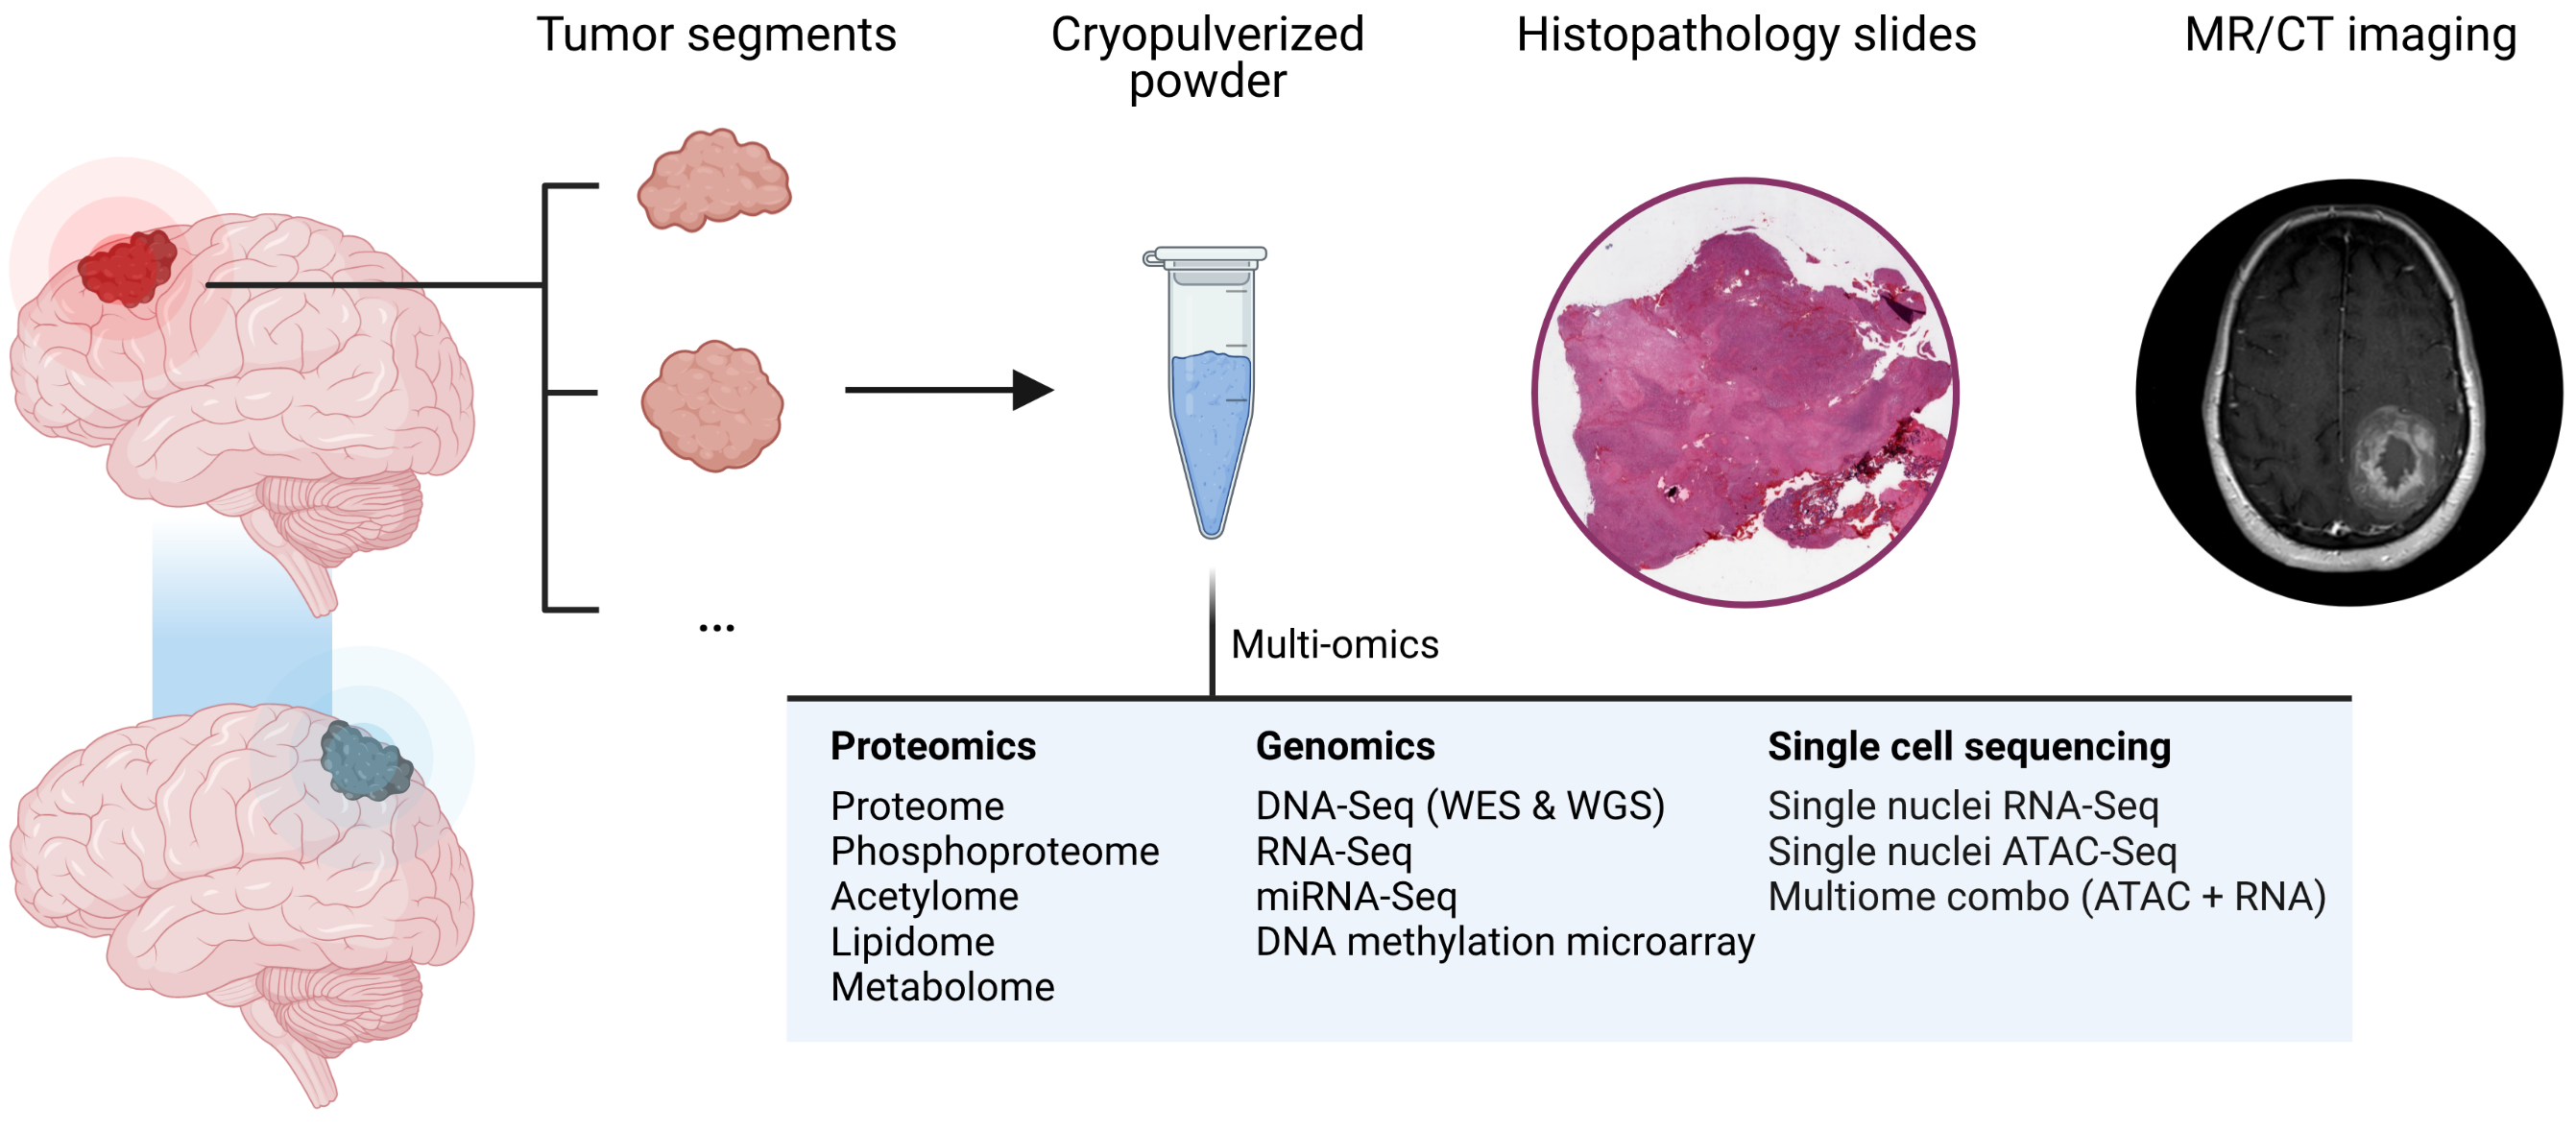
\includegraphics[width=1\linewidth]{figures/chap01_intro/cptac_gbm_multi-omics.png}
    \caption[Overview of the CPTAC GBM data collection and study design.]{%
        Overview of the CPTAC GBM data collection and study design.
        \sourceatright[2em]{\footnotesize Created with BioRender.com}
    }
    \label{fig:intro-cptac-gbm-study design}
\end{figure}


